\documentclass[12pt]{article}
%%% DOCUMENT FORMATTING %%%
\usepackage[margin=1in]{geometry}
\usepackage{enumitem}
\setlength{\parindent}{0pt}
\newcommand{\disp}{\displaystyle}
\usepackage{multicol}

%%% HEADER %%%
\usepackage{fancyhdr}
\pagestyle{fancy}
\fancyhf{}
\lhead{MATH 1080}
\rhead{Vagnozzi}
\cfoot{\thepage}

%%% MATH NOTATION & SYMBOLS %%%
\usepackage{amssymb}
\usepackage{amsmath}
\newcommand{\R}{\mathbb{R}}
\newcommand{\N}{\mathbb{N}}
\newcommand{\Z}{\mathbb{Z}}
\newcommand{\lp}{\left(}
\newcommand{\rp}{\right)}
\newcommand{\ls}{\left[}
\newcommand{\rs}{\right]}
\newcommand{\lb}{\left\{}
\newcommand{\rb}{\right\}}
\newcommand{\arccot}{\text{arccot}}
\newcommand{\arccsc}{\text{arccsc}}
\newcommand{\arcsec}{\text{arcsec}}
\DeclareSymbolFont{matha}{OML}{txmi}{m}{it}% txfonts
\DeclareMathSymbol{\varv}{\mathord}{matha}{118} 

%%% TABLES %%%
\usepackage{colortbl}

%%% GRAPHS %%%
\usepackage{tikz}
\usepackage{pgfplots}
\pgfplotsset{compat=1.15}
\usepgfplotslibrary{fillbetween}
\usetikzlibrary{angles,quotes}

%%% ENVIRONMENTS %%%
\newcommand{\Example}{\paragraph{\Writinghand \hspace{0.1mm} Example.}}
\newcommand{\Examples}{\paragraph{\Writinghand \hspace{0.1mm} Examples.}}
\newcommand{\ExampleCont}{\paragraph{\Writinghand \hspace{0.1mm} Example (continued).}}
\newcommand{\ExamplesCont}{\paragraph{\Writinghand \hspace{0.1mm} Examples (continued).}}

\newcommand{\boxenv}[2]{
	\fbox{
	\begin{minipage}{0.97\textwidth}
	\vspace{2mm}	
	\paragraph{#1} #2
	\vspace{2mm}
	\end{minipage}
	}}

%%% FUN THINGS %%%
\newcommand*\tc[1]{\tikz[baseline=(char.base)]{
            \node[shape=circle,draw,inner sep=2pt] (char) {#1};}}
\usepackage{marvosym}

%%% MISC %%%
\usepackage{hyperref}


\setcounter{page}{174}

\begin{document}
\section*{12.3: Calculus in Polar Coordinates}

\boxenv{Learning Objectives.}{Upon successful completion of Section 12.3, you will be able to\dots
		
	\begin{itemize}[leftmargin=6mm]
		\item Answer conceptual questions involving calculus in polar coordinates.
		\item Find the slope of the line tangent to a polar curve at a given point.
		\item Find the points at which a polar curve has horizontal or vertical tangent lines.
		\item Find intersection points for two polar curves.
		\item Find the area of a region bounded by polar curves.
		\item Find the lengths of polar curves.
	\end{itemize}
	\vspace{-4mm}
}

\vspace{5mm}

\subsection*{Tangents to Polar Curves}

Given a polar curve $r=f(\theta)$, how do we find $\dfrac{dy}{dx}$?

\vfill

\Example Let's consider the polar curve $r=1+\cos\theta$. Find the slope of the line tangent to the curve at $\theta=\dfrac{\pi}{2}$.

\vfill
\vfill

\newpage

\boxenv{Tangents to Polar Curves.}{The slope $\dfrac{dy}{dx}$ of the line tangent to a polar curve $r=f(\theta)$ is

$$\dfrac{dy}{dx}=\dfrac{dy/d\theta}{dx/d\theta}.$$

\vspace{5mm}

\textbf{Horizontal tangents} occur where \underline{\hspace{33mm}}, provided that \underline{\hspace{33mm}}.

\vspace{5mm}

\textbf{Vertical tangents} occur where \underline{\hspace{35mm}}, provided that \underline{\hspace{35mm}}.

 }
 
\vspace{15mm}

\Example Let's again consider the polar curve $r=1+\cos\theta$. Find the points $(r,\theta)$ where the graph has horizontal or vertical tangents.

\newpage

\subsection*{Area of a Polar Region}

\textbf{Note:} The area of the sector of a circle is $A=\dfrac{1}{2}r^2\theta$.

\vspace{50mm}

Let $R$ be the region bounded by $r=f(\theta)$ between $\theta=a$ and $\theta=b$ where $f$ is positive and continuous and $0<b-a\leq 2\pi$. How can we find the area of this region?

\newpage

\Example Consider the rose curve $r=4\sin(3\theta)$ traced out on the interval $[0,\pi]$.

\begin{enumerate}

\item[(a)] Sketch the polar curve.

\begin{flushright}
\begin{tikzpicture}
    \begin{axis}[
       	axis x line=center,
       	xmax=1.45, xmin=-1.45,
       	xtick=\empty,
       	axis y line=center,
       	ymax=1.25, ymin=-1.25,
       	ytick=\empty,
%       	xlabel=$x$,ylabel=$y$,
       	axis line style=<->
    ]
%	\addplot [domain=0:2*pi,samples=1000,color=blue,thick]({(cos(deg(x)))^3},{(sin(deg(x)))^3});
    \end{axis}
\end{tikzpicture}
\end{flushright}

\vspace{10mm}

\item[(b)] Set up a few different integrals that represent the area of one petal of the rose curve.

\vfill
\vfill

\item[(c)] Evaluate one of the representations above to determine the area enclosed by one petal.

\vfill
\end{enumerate}

\newpage

\Example Consider the region that lies inside $r=3\cos\theta$ and outside $r=1+\cos\theta$. Set up a few different integrals that could represent the area of this region.

\begin{flushright}
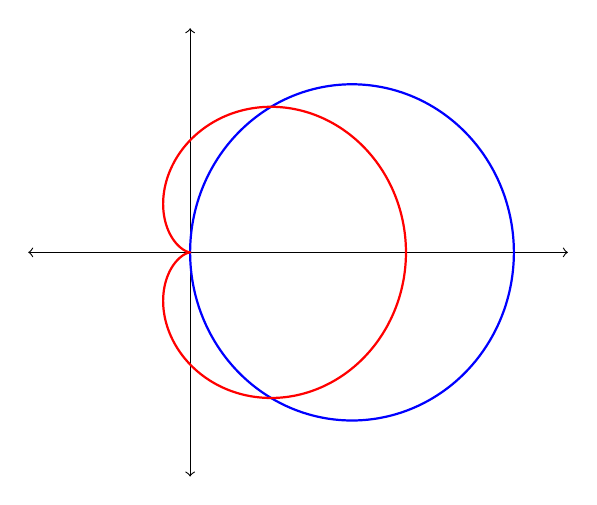
\begin{tikzpicture}
    \begin{axis}[
       	axis x line=center,
       	xmax=3.5, xmin=-1.5,
       	xtick=\empty,
       	axis y line=center,
       	ymax=2, ymin=-2,
       	ytick=\empty,
%       	xlabel=$x$,ylabel=$y$,
       	axis line style=<->
    ]
	\addplot[domain=0:180,samples=1000,color=blue,thick,data cs=polar] (x,{3*cos(x)}); 
	
\addplot[domain=0:360,samples=1000,color=red,thick,data cs=polar] (x,{1+cos(x)}); 

    \end{axis}
\end{tikzpicture}
\end{flushright}

\newpage

\Example Set up the integral(s) representing the area inside the larger loop and outside the smaller loop of $r=\dfrac{1}{2}+\cos\theta$.


\begin{flushright}
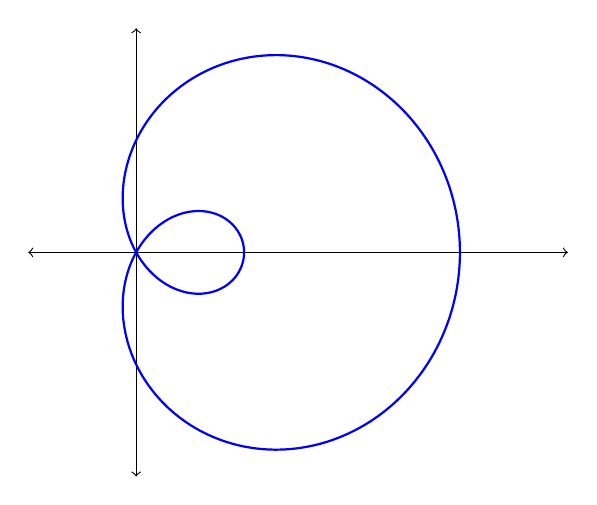
\begin{tikzpicture}
    \begin{axis}[
       	axis x line=center,
       	xmax=2, xmin=-0.5,
       	xtick=\empty,
       	axis y line=center,
       	ymax=1, ymin=-1,
       	ytick=\empty,
%       	xlabel=$x$,ylabel=$y$,
       	axis line style=<->
    ]

\addplot[domain=0:360,samples=1000,color=blue,thick,data cs=polar] (x,{0.5+cos(x)}); 

    \end{axis}
\end{tikzpicture}
\end{flushright}

\newpage

\subsection*{Polar Arc Length}

\boxenv{Polar Arc Length.}{The length of a curve with polar equation $r=f(\theta)$, $a\leq\theta\leq b$ is
$$L=\disp\int_a^b\sqrt{r^2+\left(\dfrac{dr}{d\theta}\right)^2}\,d\theta.$$}

\Example Find the length of the polar curve $r=2\cos\theta$, $0\leq\theta\leq\pi$. 
\end{document}